\scanpage{48}
Pour le voir, on est ramené par un dévissage facile, [utilisant l'existence d'une \unsure{suite} exacte
\[
 0-P'-F'-\widetilde F'\unsure{\longrightarrow|-}Q'-0
\]
où $\operatorname{Supp}P'\subset Y'$, $\operatorname{supp} Q'\subset Y'$, $\dim\operatorname{supp}P'\leq0$, $\dim\operatorname{supp}Q'\leq1$, et $\operatorname{prof}\widehat F'_{x'}$ en tt pt fermé de $X'$ --- pas seulem$^{\mathrm{t}}$ de $X'-Y'$ ! --- dévissage qui est une question purement locale sur le schéma de \uline{Jacobson} $X'$] au cas où on a $\operatorname{prof},F_x\geq2$ \deleted{D'ailleurs, si} pour \uline{tt $x\in X'$}. Soit d'ailleurs $K'$ le noyau de la multiplication par $t^n$ \deleted{\unsure{dans} $F_x$} ($n$ \unsure{grand}) \unsure{on a|sur|alors}
\[
 0-K'-F'-G'-0
\]
\deleted{\unsure{avec|alors} $G'$} $t$- \deleted{est} $G'$-régulier. On a

\figure{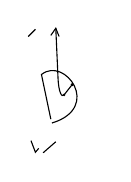
\begin{tikzpicture}[x=0.7cm,y=0.7cm]
\draw (0.18,0.31)--(0.01,1.12) .. controls (0.43,1.46) and (1.12,0.52) .. (0.20,0.24);
\draw (0.27,1.96)--(0.31,1.07) .. controls (0.32,0.79) and (0.38,0.70) .. (0.42,0.75)--(0.57,0.94);
\draw (0.18,1.83)--(0.27,1.96)--(0.33,1.81);
\fill (0.42,0.75) circle (.025) (0.57,0.94) circle (.032);
\draw (-.23,1.81)--(-.10,1.94); \draw (-.18,-.08)--(-.10,-.29)--(-.04,-.22);
\draw (.04,-.30)--(.27,-.10);
\end{tikzpicture}}

\figure{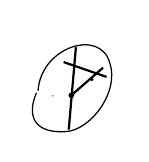
\begin{tikzpicture}[x=.65cm,y=.65cm]
\draw[line width=.45pt] (-.64,.13) .. controls (-.58,.99) and (.57,1.35) .. (.76,.68) .. controls (.96,.11) and (.38,-.66) .. (-.12,-.67) .. controls (-.80,-.7) and (-.83,-.27) .. (-.67,.09);
\draw[line width=.8pt] (-.04,-.63)--(.10,.98) (-.14,.69)--(.70,.40) (.01,.04)--(.63,.58);
\fill (.01,.04) circle (.055) (.41,.35) circle (.038) (-.35,.03) circle (.014);
\end{tikzpicture}}
\margin{$A\quad\widehat A_{\unsure{\mathfrak p|\Phi|p}}$}
\diagram{\begin{tikzcd}[ampersand replacement=\&,column sep=small]
0\arrow[r,no head]\&\Gamma K'\arrow[r]\arrow[d,"\sim"]\&\Gamma F'\arrow[r,no head]\arrow[d,"\unsure{\cdot|.}"]\&\Gamma G'\arrow[r,no head]\arrow[d,"\sim ?"]\&H^1 K'\arrow[d,"\sim"]\\
0\arrow[r]\&\Gamma\widehat K'\arrow[r,no head]\&\Gamma\widehat F'\arrow[r,no head]\&\Gamma\widehat G'\arrow[r,no head]\&H^1\widehat K'
\end{tikzcd}}
On est ramené au cas où $\unsure{G|t}$ \unsure{est|n'est} un div. de $0$.

\noindent\rule{\linewidth}{0.3pt}
% archive sheet number: 47
